% Define the module top matter
% This gets used to create the chapter title page
% NOTES:
%  * When multiple people have authored or contributed to the module, simply use a LaTeX line break
%    (a double-backslash: \\) at the end of each person.
%  * If you don't want this information shown on the module chapter page, simply remove the lines
%    within the \setModuleAuthors{} and \setModuleContributions{} environments
\setModuleTitle{Introduction to Nextflow}
\setModuleAuthors{%
  Rados{\l}aw Suchecki \mailto{rad.suchecki@csiro.au}
}
\setModuleContributions{
Nathan S. Watson-Haigh \mailto{nathan.watson-haigh@adelaide.edu.au}
}

% BEGIN: Module Title Page
% This simply uses the above information and creates a module chapter page
% NOTES:
%  * The chapter page will always appear on odd numbered page
\chapter{\moduleTitle}
\newpage
% END: Module Title Page


% BEGIN: KLOs
% Key Learning Outcomes (KLOs) are an important aspect of any learning/training. They provide
% valuable infomation about what the trainee will have learned, what they will be able to do or know
% abouti at the end of the module. Unlike objectives which are more trainer oriented, KOLs are
% focused on the learner.
% At the end of the module, the KLOs can be used to develop criteria for writing an assessment to
% see if the trainees knowledge/skills have improved as a result of the module.
%
% Search online for information on how to write KLOs. e.g.
% http://www.teaching-learning.utas.edu.au/__data/assets/word_doc/0014/23333/Learning-outcomes-v9.1.doc
\section{Key Learning Outcomes}

After completing this module the trainee should be able to:
\begin{itemize}
  \item Install Nextflow and execute an existing Nextflow workflow locally
  \item Modify the workflow to allow its execution on a compute cluster
  \item Write simple Nextflow process definitions and connect them with channels
  \item Apply operators to transform items emitted by a channel
  \item Leverage Nextflow's implicit parallelisation to process multiple data chunks independently
\end{itemize}
% END KLOs

% BEGIN: Resources Used
% This section can be used to describe the tools and data used during the module. It helps to act as
% a future reference to the trainee
\section{Resources Required}

For the purpose of this training you need access to:

\begin{itemize}
  \item A compute cluster with the \texttt{module} command available to you for loading software
  \item \url{https://sylabs.io/singularity/}{Singularity} - available as a module on the above cluster
  \item \url{https://www.anaconda.com/distribution/}{conda} - available as a module on the above cluster
\end{itemize}


\subsection{Tools Used}
\begin{description}[style=multiline,labelindent=0cm,align=left,leftmargin=0.5cm]
  \item[Nextflow]\hfill\\
    \url{https://nextflow.io}
  \item[Graphviz]\hfill\\
    \url{https://www.graphviz.org}
\end{description}

\section{Useful Links}

\begin{description}[style=multiline,labelindent=0cm,align=left,leftmargin=0.5cm]
  \item[Nextflow Documentation]\hfill\\
    \url{https://www.nextflow.io/docs/latest/index.html}
  \item[Nextflow Patterns]\hfill\\
    \url{http://nextflow-io.github.io/patterns/}
  \item[Slurm Documentation]\hfill\\
    \url{https://slurm.schedmd.com/documentation.html}

\end{description}

\newpage
% END: Resources Used

% BEGIN: Introduction
\section{Introduction}


\newpage

\section{Setting Up Your Environment}

For the purpose of the workshop we will be working on the head node of an HPC cluster running \href{https://slurm.schedmd.com/documentation.html}{Slurm}.
This is the most likely infrastructure that fellow bioinformaticians already find themselves using
on a regular basis. We also assume that the cluster provides the \texttt{module} command for you to
load software and the modules Java and Singularity are available to use.

The execution of the Nextflow workflow will take place on the cluster head node with jobs
being submitted to Slurm for queuing and processing. From the head node, Nextflow will monitor the
submitted jobs for their completion status and submit new jobs as dependent jobs complete successfully.


\subsection{Connect to the Cluster Head Node}

\begin{steps}
First up, lets connect to the head node of the HPC cluster using \texttt{ssh}.

\emph{See your local facilitator for connection details. You should have one user account per person.}

\end{steps}

\subsection{Install nextflow}


\begin{steps}
\begin{lstlisting}
# Load the Java module on your cluster
# If it's unavailable contact the cluster sysadmin
module load openjdk-1.8.0_202-b08-gcc-5.4.0-sypwasp 

# Download and install nextflow executable
curl -s https://get.nextflow.io | bash

# You should now be able to run it
./nextflow help
\end{lstlisting}
\end{steps}

The installation should have placed the executable in your working directory.
It is preferable to move the executable to a directory accessible via \texttt{\$PATH}, 
to be able to run \texttt{nextflow} rather than having to remember 
to type the full \texttt{/path/to/nextflow} each time you want to run it.

Depending on the system this may suffice:

\begin{steps}
\begin{lstlisting}
mkdir -p $HOME/bin
mv ./nextflow $HOME/bin
\end{lstlisting}
\end{steps}

You should now be able to run \texttt{nextflow} without specifying the location of the binary.

Let's see if it works by running a script which is nextflow's take on `hello world'.

\subsection{Hello (nextflow) world!}

\begin{steps}
\begin{lstlisting}
nextflow run rsuchecki/hello
\end{lstlisting}
\end{steps}

Nextflow will pull the \texttt{rsuchecki/hello} GitHub repository and run its main script.\\

\begin{note}
We are relying on nextflow's integration with git and git registries. 
The \textbf{alternative} would be to
\begin{verbatim}
git clone https://github.com/rsuchecki/hello.git
nextflow run hello/main.nf
\end{verbatim}
In which case the location of the cloned repository will be different to the one used by nextflow.
You will also not have access to nextflow-git integration functionality. 
\end{note}

\begin{questions}
Where do we find the local copy of \texttt{hello}? Hint: try \texttt{nextflow} commands related to pipeline sharing, such as \texttt{list} and \texttt{info}.
\begin{answer}
\begin{lstlisting}
# List local clones of remote repositories
nextflow list
# Get detailed info about a repository 
nextflow info hello #or nextflow rsuchecki/hello
\end{lstlisting}

\begin{verbatim}
 project name: rsuchecki/hello
 repository  : https://github.com/rsuchecki/hello
 local path  : /home/rad/.nextflow/assets/rsuchecki/hello
 main script : main.nf
 revisions   : 
 * master (default)
   mybranch
   slurm
   testing
   v1.1 [t]
   v1.2 [t]
\end{verbatim}
\end{answer}
\end{questions}


For now, we are mostly interested in the local path to the repository, the file name of the main script 
and its contents, which we will discuss next.


\begin{bonus}
While waiting for others to catch up, why not have a look into how you would go about pulling and removing  
local clones of remote repositories using nextflow.
\begin{answer}
\begin{lstlisting}
# remove local copy of rsuchecki/hello
nextflow drop hello
# pull rsuchecki/hello from remote without running the main script
nextflow pull rsuchecki/hello
\end{lstlisting}
\end{answer}
\end{bonus}

\begin{bonus}
What revisions (git branches or tags) are available for \texttt{nextflow-io/hello}?
How would you run a specific revision? 
\begin{answer}
\begin{lstlisting}
# Available revisions 
nextflow info hello
# Using -r/-revision, pointing to a listed tag or branch
nextflow run hello -revision v1.1
\end{lstlisting}
\end{answer}
\end{bonus}

\section{Nextflow basics}

\subsection{Processes and channels}


\begin{itemize}
\item \emph{process} -- a wrapper for a language-agnostic script which ensures isolation of the executed code.
\item \emph{channel} -- an asynchronous\footnote{send operation completes immediately, receiving stops the receiving process until the message has arrived} FIFO queue which facilitates data flow to/from/between processes by linking their outputs/inputs.
\end{itemize}


\begin{figure}[H]
\centering
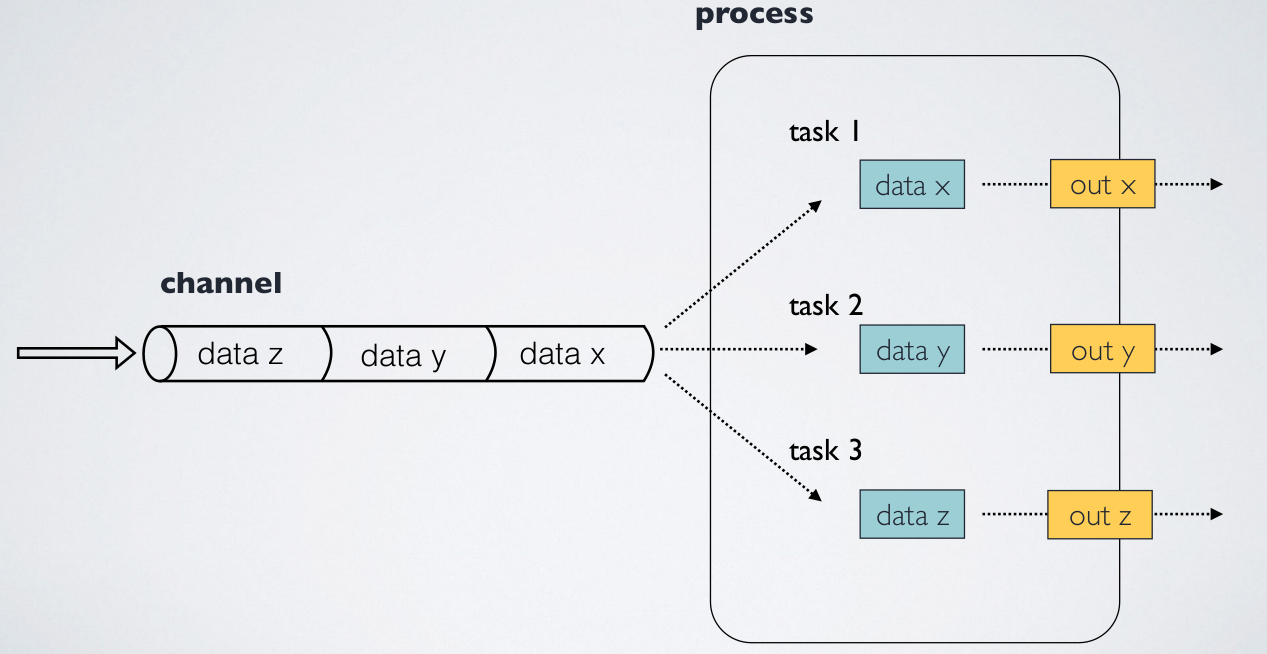
\includegraphics[width=.8\textwidth]{handout/channel-process.png}
\caption{Nextflow building blocks: a \emph{channel} ``feeding'' a processes. 
A \emph{task} is an instance of a process. An isolated task is created for each emission (data chunk) from the input channel. Credit: Evan Floden}
\label{fig:proc-chn}
\end{figure}


\subsection{The main script}

A nextflow script file name can be anything but in most cases it is best to stick to the default \texttt{main.nf}. 
The main script for the `hello' example is as follows:


\begin{lstlisting}
#!/usr/bin/env nextflow
echo true

cheers = Channel.from 'Bonjour', 'Ciao', 'Hello', 'Hola'

//setting default value, to be modified at runtime 
params.world = 'world' 

process sayHello {
  input:
    val x from cheers
  script:
    """
    echo '$x $params.world!'
    """
}
\end{lstlisting}



A channel called \texttt{cheers} is created and emits each of the listed strings separately. 
A separate instance of the process \texttt{sayHello} is executed for each emission. 

\begin{note}
The contenet of the above script can be broken down as follows:
\begin{itemize}
  \item The shebang line (line 1) is optional.
  \item Setting \texttt{echo true} will output \texttt{stdout} of (every) process to the terminal - not advised for real world applications.
  \item \texttt{Channel.from(some\_list)} creates a channel emitting the list elements one by one.
  \item \href{https://www.nextflow.io/docs/latest/process.html}{Process} definition (lines 6-13)
  \begin{itemize}
    \item Input block (lines 7-8)
    \item Script block (lines 9-12)
  \end{itemize}
  \item The \texttt{\$x} in the script block is a nextflow variable local to the process, not a bash variable.
  \item Indentation is inconsequential. 
\end{itemize}
In addition \href{https://www.nextflow.io/docs/latest/process.html#directives}{process directives} could be inserted above the input block.
\end{note}


\subsection{Hello HPC!}

The nextflow hello example shown us how the \texttt{sayHello} process was executed separately for each input string as a separate \emph{task}, but all the tasks were executed locally on our cluster's head node. 
We would now like each task to be submitted as a batch job for execution on one of the compute nodes.

\begin{steps}
\begin{lstlisting}
nextflow run rsuchecki/hello -revision slurm
\end{lstlisting}
\end{steps}

This is the modified version of the \texttt{main.nf} script. 
Submission to Slurm was achieved by adding \texttt{executor 'slurm'} directive to the process definition.

\begin{lstlisting}
#!/usr/bin/env nextflow
echo true

cheers = Channel.from 'Bonjour', 'Ciao', 'Hello', 'Hola'

//setting default value, to be modified at runtime 
params.world = 'world' 

process sayHello {
  executor 'slurm'

  input:
    val x from cheers
  script:
    """
    echo "$x $params.world from \$HOSTNAME on Slurm!"
    """
}
\end{lstlisting}

You might also have noticed that we have modified the script block so that the messages printed to the terminal include the name of the compute node on which a given task is executed. 

\begin{warning}
Note the difference between how nextflow variables (\texttt{\$x,\$params.world}) and bash variables (\texttt{\$HOSTNAME})are included in the script block.
There are alternative ways of including variables in scripts for execution by nextflow processes which may be more convenient if your script contains multiple special characters.
\end{warning}


\subsection{Hello task caching!}

When the pipeline is launched with the \texttt{-resume} option, 
any attempt to execute already executed process with the same inputs,
will cause the process execution to be skipped, 
producing the stored data as the output.

In this toy example we do not specify any outputs 
but the `hello` messages printed to the terminal 
reflect this behaviour.

%The caching feature generates a unique key by indexing the process script and inputs. 
%This key is used to identify the outputs produced by the process execution.

\begin{steps}
\begin{lstlisting}
nextflow run rsuchecki/hello -revision slurm -resume
\end{lstlisting}
\end{steps}

To avoid unintentionally re-computing long running tasks you may consider 
always running your pipelines with \texttt{-resume} and only omitting it
on rare occasions when you want to re-compute the results
even though inputs have not changed. 

\url{https://www.nextflow.io/docs/latest/process.html#cache}

\subsection{Hello command line options}

Single-dashed options are reserved for nextflow engine (\texttt{-resume, -revision, -ansi-log false} etc). 
The double-dashed options are all yours and you are free to use them for your workflow. 
When you \texttt{nextflow run some\_script.nf --foo bar}, 
the value of the parameter (`bar')
will be accessible in \texttt{main.nf} as \texttt{params.foo}
and within a script block as \texttt{\$params.foo}.

\begin{steps}
In the `hello' example we use \texttt{params.world} which by default is set to `word', so lets try to use an alternative string.

\begin{lstlisting}
nextflow run rsuchecki/hello -revision slurm --world Mundo
\end{lstlisting}
\end{steps}

\subsection{Goodbye Hello}


Nextflow facilitates but does not enforce separation of workflow logic from the configuration
of compute and software environments as well as from other properties of the workflow.  
As such, you \textit{could} get by developing nextflow workflows without worrying about that 
aspect -- but you would be missing a lot in terms of flexibility, extensibility, portability and more

Nextflow looks for workflow configuration primarily in \texttt{nextflow.config} file, and additional config files can be included. Unsurprisingly the `hello' example does not require much configuration,
we would also like to crunch some real, albeit small, data.


\begin{steps}
\\This is mostly symbolic
\begin{lstlisting}
nextflow drop rsuchecki/hello
\end{lstlisting}
\end{steps}


Let's have a play with a slightly more practical workflow.




\newpage

\section{Example workflow}

We are going to work with an example Nextflow workflow to demonstrate how they are run, 
improve your understanding of \emph{processes} and \emph{channels} and finally introduce\ \emph{operators}, which are applied to channels to shape and direct flowing data.


This example workflow consists of the following steps:

\begin{itemize}
  \item Running FastQC across the raw reads
  \item Aggregating the raw read FastQC reports using MultiQC
  \item Performing adapter, quality, and read length filtering using Trimmomatic
  \item Running FastQC across the QC'd reads
  \item Aggregating the QC read FastQC reports using MultiQC
  \item Indexing the reference FASTA file
  \item Performing a \texttt{bwa-mem} read alignment
\end{itemize}


\begin{steps}
Although not necessary for simply running the pipeline, in the training context it makes sense to start by cloning the workflow repository and moving to the directory.

\begin{lstlisting}
git clone https://github.com/csiro-crop-informatics/nextflow-embl-abr-webinar.git example_workflow
cd example_workflow
git checkout noslurm
git branch
\end{lstlisting}

This time, in addition to \texttt{main.nf} we have a separate script which downloads the required data sets, which include a small reference FASTA file and 16 pairs of FASTQ files, each for a different bread wheat accession. 


\begin{lstlisting}
nextflow run setup_data.nf
\end{lstlisting}

alternatively, you should be able to link to the data on the shared drive

\begin{lstlisting}
ln -s /shared/data
\end{lstlisting}

%# or
%nextflow run csiro-crop-informatics/nextflow-embl-abr-webinar/setup_data.nf -revision workshop

If successful, we could now try to run the workflow...

\begin{lstlisting}
nextflow run main.nf
\end{lstlisting}

\begin{warning}
This is expected to fail.\\
Unless all the software required by the pipeline is available on the \texttt{\$PATH},
which we don't expect, the pipeline should terminate with an error.
The output information may help you identify the cause. 
Try to relate the error message to the relevant section of the main script (\texttt{main.nf}). 
\end{warning}
\end{steps}

\begin{questions}
Which process has failed?
What was the underlying cause?
\begin{answer}
The cause was likely ``\texttt{command not found}'' and it may have been any of the processes for which the software tool is not available.
Example:
\begin{lstlisting}
Error executing process > 'fastqc_raw (Xiaoyan)'

Caused by:
  Process `fastqc_raw (Xiaoyan)` terminated with an error exit status (127)

Command executed:

  fastqc  --quiet --threads 1 *

Command exit status:
  127

Command output:
  (empty)

Command error:
  .command.sh: line 2: fastqc: command not found

Work dir:  /tmp/nextflow-embl-abr-webinar/work/15/505ea816d2411e68ea253ee126c181
\end{lstlisting}
\end{answer}
\end{questions}


There are two main issues with executing this workflow as is, 
\begin{enumerate}
 \item Third-party software tools have not been made available to the workflow.
 \item We are trying to run the entire workflow on the cluster's head node.
\end{enumerate}

There are different ways in which these issues could be addressed, for example using process 
\emph{directives} at the top of each process definition. 
Depending on your cluster configuration this could be for example:
\begin{lstlisting}
process foo {
  executor 'slurm' 
  module 'samtools/1.9' 
  //further code omitted 
\end{lstlisting}

This is a perfectly valid syntax, which can be convenient, particularly during pipeline development, 
but for more portable workflows it is preferable to keep compute and software environment configuration 
separate from pipeline logic -- in simple terms not in the workflow script (\texttt{main.nf}).

\subsection{The config file(s) and profiles}

Workflow configuration belongs in \texttt{nextflow.config} file. 
Transferring the above mention \emph{directives} from process definitions in \texttt{main.nf} 
to \texttt{nextflow.config} would make things slightly better, e.g.

\begin{lstlisting}
#nextflow.config

process.executor = 'slurm' 
process.module = 'samtools/1.9' 
\end{lstlisting}

or using the preferred syntax

\begin{lstlisting}
process {
  executor = slurm
  module = 'samtools/1.9'
}
\end{lstlisting}


This is however still a bit rigid. 
\begin{itemize}
\item You may be developing your pipeline on a local machine or a server where software modules are not available. 
\item If developing directly in the cluster environment, you may prefer your quick test runs to happen either on the head node or in an interactive session you are using, rather than always having jobs submitted to sit in the always-busy cluster queue.
\end{itemize}



Nextflow enables the definition of \emph{profiles} which make it easy to run a workflow 
with different configuration settings, including, but not limited to executors and software environment.

For our pipeline we have defined several \emph{profiles}, which allow us to execute the logic in \texttt{main.nf} while providing the required software either by creating a \texttt{conda} environment or by using Docker of Singularity containers where the conda environment has already been captured. 

\subsubsection{Relevant profiles}


Identify the profile definitions in \texttt{nextflow config}. The ones most immediately relevant are:
\begin{lstlisting}
profiles {
  //SOFTWARE
  conda {
    process {
      conda = "$baseDir/conf/conda.yaml"
    }
  }
  singularity {
    process {
      container = 'shub://csiro-crop-informatics/nextflow-embl-abr-webinar' 
    }
    singularity {
      enabled = true
      autoMounts = true
      cacheDir = "singularity-images"  
    }
  }
}
\end{lstlisting}



As you can see, Nextflow makes it really easy to %use different executors and the configuration of 
define software environment via Singularity or Conda\footnote{We also have a docker profile which you may find useful if you decide to run the workflow on your machine}. 
%is also straightforward. 

%You could now run the workflow with Singularity on the head node (generally not advised), 
%or by starting an interactive session on one of the compute nodes.
%
%\begin{steps}
%\begin{lstlisting}
%srun --pty bash
%\end{lstlisting}

%and once you get onto one of the compute nodes 


Given that Singlularity is available on our cluster, let's start by using that profile,
as the most robust way of setting up the software environment.



We will need Singularity for nextflow to be able to pull the container image from Singularity Hub and run the containerised software. 
By default the pipeline will process reads for a single accession -- our head node should be able to handle this. 

\begin{steps}
\begin{lstlisting}
# Load the Singularity module 
# If it is unavailable contact the cluster sysadmin

module load singularity-3.2.1-gcc-5.4.0-tn5ndnb

# Run the workflow

nextflow run main.nf -profile singularity
\end{lstlisting}
\end{steps}
%# Release the resources - leave the interactive session.
%exit

This is sufficient when running a workflow locally, in an interactive session or on a standalone server. 
The next step is to get nextflow to make use of the HPC batch submission system, to be able to run the full workflow 
without unleashing your sysadmins wrath.\\ 

\begin{steps}
Edit \texttt{nextflow.config}. Your task is to add a \texttt{slurm} profile which will set the appropriate executor. 
\end{steps}

\begin{questions}
What is your \texttt{slurm} profile configuration and where do you place it in \texttt{nextflow.config}?
\begin{answer}
The following code should be placed within the \texttt{profiles\{\}} block in \texttt{nextflow.config}.
\begin{lstlisting}
  slurm {
    process {
      executor = 'slurm'
    }
  }
\end{lstlisting}
\end{answer}
\end{questions}

%\begin{questions}
%\begin{answer}
%\end{answer}
%\end{questions}


There are of course many setting that can and in some cases must be set -- refer to 
\href{https://www.nextflow.io/docs/latest/executor.html}{executors section of Nextflow documentation}\footnote{\url{https://www.nextflow.io/docs/latest/executor.html}}. 
For running real-life pipelines in a cluster environment you will also use 
\href{https://www.nextflow.io/docs/latest/process.html#directives}{directives} \footnote{\url{https://www.nextflow.io/docs/latest/process.html\#directives}}
controlling the resources (\texttt{cpus, memory, time}) requested for each job. Other possibly relevant directives include \texttt{queue} and \texttt{scratch}.



\subsection{Cluster run}


To avoid running the workflow on our head node or in an interactive session, we will use the \texttt{slurm} profile you have defined\footnote{If you are struggling and can't get help, try: \texttt{git stash \&\& git checkout workshop}}. 
As before, the software environment will be handled via the \texttt{singularity} profile. 
For that, we will need Singularity on the head node for nextflow to be able to pull the container image from Singularity Hub (we could also use a locally stored image). Singularity will also be required on the compute nodes which will run the individual tasks, but this should happen seamlessly if an appropriate module is loaded on the head node, otherwise the required module would also have to be specified in the workflow configuration files. 

\begin{steps}
By default a single accession will be processed. 
You may use the \texttt{-resume} flag to avoid re-computing already existing results. 


\begin{lstlisting}
# Load the Singularity module on your cluster
# If it is unavailable contact the cluster sysadmin

module load singularity-3.2.1-gcc-5.4.0-tn5ndnb

# Run the workflow

nextflow run main.nf -profile slurm,singularity -resume
\end{lstlisting}
\end{steps}

%\begin{lstlisting}
%nextflow run main.nf -profile slurm,singularity -resume
%\end{lstlisting}
%\end{steps}


\subsection{Under the hood}

If you think you are ready to look under the hood and try to work out how nextflow stages process inputs, wraps process script blocks and submits them to the cluster, here is a start. 

\begin{advanced}
\begin{lstlisting}
# Remove the work directory to limit the number of task directories to look at
rm -r work
# Re-run for a single sample
nextflow run main.nf -profile slurm,singularity
# Take a peak
ls -la work/ | less
# or
tree -ah work/ | less
\end{lstlisting}

Each task is executed in a separate directory and every abbreviated hash displayed in the terminal can be related to a specific sub-directory of \texttt{./work},\\ such as
\texttt{work/d2/c4517b0a81f61ceca29ec355ddeaa6/} in which you may find

\begin{lstlisting}
# NF generated files
.command.begin
.command.err
.command.log
.command.out
.command.run
.command.sh
.command.trace
.exitcode

# Output file
H45.bam

# Symlinks to input files
H45_R1.paired.fastq.gz
H45_R2.paired.fastq.gz
reference.fasta.gz.amb
reference.fasta.gz.ann
reference.fasta.gz.bwt
reference.fasta.gz.pac
reference.fasta.gz.sa
\end{lstlisting}

Identify and investigate hidden file (starting with dot) containing the executed script and the one containing cluster and container handling. 

%\begin{questions}
%
%\begin{answer}
%
%\end{answer}
%\end{questions}

\end{advanced}


\subsection{Cluster run - all accessions}

We have successfully submitted workflow to the cluster. 

To be sure, feel free to re-run it again (and again, and again...) 
with \texttt{-resume} to avoid wasting CPU cycles.

\begin{steps}
\begin{lstlisting}
nextflow run main.nf -profile slurm,singularity -resume
\end{lstlisting}
\end{steps}

If all went well, the workflow successfully processed a single accession, 
let's have a closer look at the script to better understand how it handles 
the inputs before we proceed to run it on all the accessions.

\begin{questions}
In \texttt{main.nf} we create a channel which reads pairs of FASTQ files from a sub-directory of the \texttt{./data}. We then apply some operators. 
\begin{verbatim}
Channel.fromFilePairs("data/${region}/*_R{1,2}.fastq.gz")
  .take ( params.take == "all" ? -1 : params.take ) 
  .into { readPairsChannelA; readPairsChannelB } 
\end{verbatim}
1. Identify the two operators, refer to 
\href{https://www.nextflow.io/docs/latest/operator.html}{nextflow documentation}\footnote{\url{https://www.nextflow.io/docs/latest/operator.html}}
as required and explain the purpose of each of the two operators.\\
\begin{answer}
\texttt{.take($n$)} limits the number of emissions from the channel to the first $n$ items. \\
\texttt{.into\{ $ch_1;ch_2;...;ch_n$ \}} creates channels $ch_1,ch_2,...,ch_n$ and connects source channel to the newly created channels, so that every emission is sent through each new channel.
\end{answer}

2. How can you run the workflow for more than one accession? How about all of them? Recall that workflow parameters use double-dash syntax. Run the relevant commands.  
\begin{answer}
\begin{lstlisting}
nextflow run main.nf -profile slurm,singularity -resume --take 2
nextflow run main.nf -profile slurm,singularity -resume --take all
\end{lstlisting}
\end{answer}
%3. Investigate \texttt{main.nf} to identify the processes which consume \texttt{readPairsChannelA} and \texttt{readPairsChannelB}. \\
%
%Q????
%
\end{questions}

\subsubsection{Monitoring your jobs on our cluster}

\begin{note}
You can monitor your job(s) in the slurm queue using the slurm command \texttt{squeue}:

\begin{lstlisting}
squeue --user ${USER}
\end{lstlisting}

For convenience you are also provided with the \texttt{sq} function which produces nicer output and by default only shows your own jobs:

\begin{lstlisting}
sq

# Someone elses jobs
sq --user ${SOMEONE_ELSE}
\end{lstlisting}

If you want to see all jobs in the queue:

\begin{lstlisting}
squeue
\end{lstlisting}

\end{note}

\begin{bonus}
For an optional exercise you may try to re-run the workflow with \texttt{conda}.
For that, you'll need to find and load a conda module before re-running the workflow with appropriate profile. Don't forget to use the \texttt{-resume} flag.
\begin{answer}
\begin{lstlisting}
# Find the appropriate module name
module av -l 2>&1 | grep conda

# Load the module
module load miniconda3-4.6.14-gcc-5.4.0-kkzv7zk

# Run with conda
nextflow run main.nf -profile conda,slurm --take all -resume

\end{lstlisting}
\end{answer}

If you remembered to use \texttt{-resume}, why do you think it appeared to not make a difference?

\begin{answer}
We have switched from singularity to conda so the software environment has changed.  
\end{answer}


\end{bonus}


\begin{figure}[H]
\centering
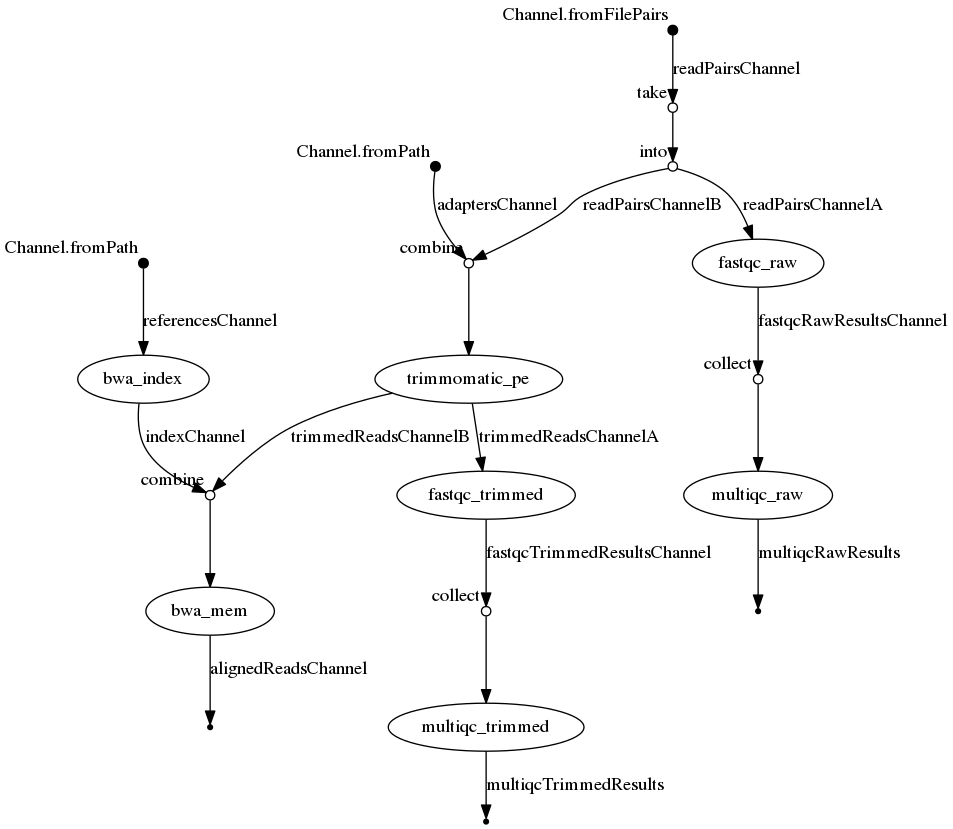
\includegraphics[width=\textwidth]{handout/flowchart.png}
\caption{The example workflow}
\label{fig:dag}
\end{figure}


\begin{questions}
Investigate \texttt{main.nf} alongside Figure~\ref{fig:dag}. 

Which \href{https://www.nextflow.io/docs/latest/operator.html}{nextflow operators}\footnote{\url{https://www.nextflow.io/docs/latest/operator.html}}, in addition to the previously discussed, are used and for what purposes? 

\begin{answer}
The \texttt{.combine()} operator outputs all combinations of items emitted by two channels. This results with a downstream process to be executed for each such combination. So e.g. \texttt{bwa\_mem} will be executed for\\ $(reference, accession_1),(reference, accession_2),..,(reference, accession_n)$.

The \texttt{.collect()} operator collects all the items emitted by a channel returns the resulting \texttt{List} as a single emission. This is required e.g.\ if a process needs to be executed once with all the samples as input.
\end{answer}

\end{questions}


\subsection{Workflow outputs}

We now now each task is nicely isolated in a separate sub-directory under \texttt{work}, but how do I find my results? Was it \texttt{work/a7:fc9339a827fb4b34d2408e1c3ee29c} or maybe \texttt{work/3c:8fdf958e96b448ecb83bd7806af382}? This should be handled by applying the \href{https://www.nextflow.io/docs/latest/process.html#publishdir}{\texttt{publishDir} directive}\footnote{\url{https://www.nextflow.io/docs/latest/process.html\#publishdir}} to selected processes. As with other directives, this can be included at the top of the process block or in a configuration file using \href{https://www.nextflow.io/docs/latest/config.html#process-selectors}{process selectors}\footnote{\url{https://www.nextflow.io/docs/latest/config.html\#process-selectors}} to apply the directive to one or more relevant process. To keep things tidy-ish, we define the publishing of the outputs in a separate file 
which we \texttt{includeConfig 'conf/publish.config'} in \texttt{nextflow.config}. 

\begin{bonus}
In \texttt{conf/publish.config} we only really use the \texttt{withName} selectors. 

\end{bonus}

\section{Modify/extend the workflow}

\begin{steps}

Option 0\\
Edit \texttt{main.nf}. Your task is to add a process which will merge the bam files produced by the \texttt{bwa\_mem} process.\\ 

Option 1\\
Edit \texttt{main.nf}. Your task is to add another multiqc process which will summarize all fastqc results together, i.e. those from raw and from the trimmed data. \\
%additional 2 channels, additional process with .collect

Option 2 (advanced) \\
Add a process which will take all raw reads and all paired reads for a given sample, count the number of raw paired reads and the number of paired reads remaining after the trimming.

%\texttt{groupTuple}?\\

\end{steps}

\section{Your own workflow (TODO: replace with variant calling?)}

It is time to have a go at your own pipeline. 
Since we have some inputs and configuration files at hand, 
you can start a \texttt{own.nf} script file in the current 
directory and read the input files from \texttt{./data}. 



\begin{questions}
The simple pipeline should include the following:

\begin{itemize}
\item Code for reading FASTQ read files from \texttt{./data} individually (i.e.\ not as pairs) into a channel.
\item A process which will take a read file, count the reads and output the file name alongside the read count.
\item A way of aggregating the individual count files into a single csv file. This could be done in another process or using an operator. 
\end{itemize}

\begin{answer}

There are different ways of approaching the exercise, 
here is an example solution.
For comparison, we demonstrate the aggregating step both as a process
and using the \texttt{collectFile()} operator. 

\begin{lstlisting}
readsChannel = Channel.fromPath("data/**.fastq.gz") 

process countReads {
  input:
    file fastq from readsChannel

  output:
    file '*' into countsChannel1, countsChannel2

  """
  echo -ne "${fastq}," > count
  zcat $fastq | paste - - - - | wc -l >> count
  """
}

process aggregate {
  publishDir params.outdir

  input:
    file '*.count' from countsChannel1.collect()

  output:
    file '*.csv'

  """
  cat *.count > counts_from_process.csv
  """
}

countsChannel2.collectFile(name: 'counts_from_operator.csv', storeDir: params.outdir)
\end{lstlisting}
\end{answer}

\end{questions}
\subsection{Key concepts to cover}



\begin{itemize}
 \item channels
 \item operators
 \item processes
 \item directives
\end{itemize}

\subsection {Under the hood}



\subsection{Parametrisation}

\begin{itemize}
 \item single dash params
 \item double dash params
 \item environmental variables
\end{itemize}

% To make a paragraph appear as a "note" to the reader, simply wrap it in a "note" environment like
% this:
\begin{note}
Note that currently the default behaviour of Nextflow is to re-run an entire workflow 
unless \texttt{-resume} option is specified at run-time, in which case a previously 
executed process is not re-run if all its inputs remain unchanged.

\end{note}


\subsection{additional exercises}

\begin{enumerate}
 \item \texttt{publishDir}
 \item process selectors (optional)
\end{enumerate}


%========================
\section{Troubleshooting}
%========================

\subsection{Disconnected from the cluster?}  

\subsection{Missing modules - new shell session?}



Make sure all the required modules are loaded. 

\begin{steps}
\begin{lstlisting}
# Java - essential for nextflow
module load openjdk-1.8.0_202-b08-gcc-5.4.0-sypwasp 

# Singularity - our go to system for providing software for the example workflow
module load singularity-3.2.1-gcc-5.4.0-tn5ndnb


# If using conda 
module load miniconda3-4.6.14-gcc-5.4.0-kkzv7zk
\end{lstlisting}
\end{steps}




